
% RUN in terminal (without bibliography):
% pdflatex -output-directory=/Users/salvatorpes/Desktop/LFEUI/text/proposta /Users/salvatorpes/Desktop/LFEUI/text/proposta/prop.tex

\documentclass{article}

\author{
    \begin{tabular}{rl}
        Estêvão Gomes (ist1102650) & Sofia Nunes (ist1102633) \\
        Pedro Curvo (ist1102716) & Salvador Torpes (ist1102474)
    \end{tabular}
}

\usepackage[utf8]{inputenc}
\usepackage[english]{babel}
\usepackage[letterpaper,top=10mm,bottom=15mm,left=10mm,right=10mm,marginparwidth=1.75cm]{geometry}
\usepackage{multicol}
\usepackage{graphicx}
\usepackage{subcaption}
\usepackage{tabularx}
\usepackage{booktabs}
\usepackage{array}
\usepackage{makecell}
\usepackage{titlesec}
\usepackage{multirow}
\usepackage{amsmath}
\usepackage{makecell}
\usepackage{url}
\usepackage{csquotes}
\usepackage{caption}
\usepackage{enumitem}
\usepackage{textcomp}
\usepackage{pdflscape}
\usepackage{makeidx}
% \usepackage{tocbibind}
\providecommand{\tightlist}{\relax}
\usepackage{tocloft}
\renewcommand{\cftsecindent}{0em}
\renewcommand{\cftsubsecindent}{1em}
\renewcommand{\cftsecfont}{\bfseries}
\renewcommand{\cftsubsecfont}{\itshape}
\setlength{\cftsubsecnumwidth}{0em}

\usepackage[version=4]{mhchem}
\usepackage{hyperref} % Remove "pdftex" option here
\usepackage{float}
\usepackage{fancyhdr}
\usepackage{ragged2e}
\usepackage{xkeyval}
%\usepackage{minted}
%\usemintedstyle{manni}
\usepackage{listings}
\usepackage{amssymb}


\usepackage{xcolor}
\usepackage{tikz}

\usetikzlibrary{positioning}
\usetikzlibrary{positioning, arrows.meta}
\usepackage{adjustbox}
\usepackage{sidecap}
\usepackage{graphicx}

\usepackage{tikz-3dplot}
\usepackage{pgfplots}
\usetikzlibrary{calc, 3d, arrows}



\usetikzlibrary{shapes.geometric, arrows}


\lstset{
    language=Python,
    basicstyle=\ttfamily,
    keywordstyle=\color{blue},
    commentstyle=\color{gray},
    stringstyle=\color{orange},
    numbers=left,
    numberstyle=\tiny,
    numbersep=5pt,
    showspaces=false,
    showstringspaces=false,
    breaklines=true,
    frame=tb,
    framexleftmargin=2em,
    xleftmargin=2em,
}


%\usepackage{fontspec}

%\setmonofont{Fira Code}

\fancyhf{}
\cfoot{\thepage}
\fancyhf{} % Clear all header and footer fields
\renewcommand{\headrulewidth}{0pt} % Remove the header rule line
\cfoot{\thepage} % Set the page number in the center of the footer

\pagestyle{fancy} % Apply the fancy page style

\setlength\columnsep{20pt}

\renewcommand{\familydefault}{\sfdefault}

\newenvironment{Figure}
  {\par\medskip\noindent\minipage{\linewidth}}
  {\endminipage\par\medskip}

\makeatletter
\newenvironment{figurehere}
{\def\@captype{figure}}
{}
\makeatother

\hypersetup{
  colorlinks,
  linkcolor=blue,
  anchorcolor=black,
  citecolor=cyan,
  filecolor=cyan,
  menucolor=cyan,
  urlcolor=cyan,
  bookmarksopen=true,
  bookmarksnumbered=true
}

\makeindex


\title{\vspace{-13mm}
\includegraphics[width=15mm,scale=3]{../images/IST_Logo.png}\\ \vspace{5mm}
LFEUI - Investigation Proposal \\ \vspace{4mm} {\fontsize{24}{16}Detection of Li in Technological Materials through Nuclear Reactions} \vspace{-1mm}}
\date{November 2023}

\usepackage{sansmathfonts}
\usepackage[T1]{fontenc}
\usepackage[OT1]{fontenc}

\titleformat{\section}{\normalfont\large\bfseries}{\thesection}{1em}{}



\usepackage[style=numeric]{biblatex} % Choose your desired citation style
\addbibresource{../references/prop.bib} % Specify your .bib file

\begin{document}

\renewcommand{\arraystretch}{1.5}
\setlength{\columnseprule}{0.4pt}
\tdplotsetmaincoords{70}{110} % Set the viewing angle
\newcolumntype{M}[1]{>{\centering\arraybackslash\vspace{#1}}m{0.5\linewidth}<{\vspace{#1}}}
\newcolumntype{C}[2]{>{\centering\arraybackslash\vspace{#1}\rule{0pt}{#1}\hspace{0pt}}m{#2}}
\newcolumntype{w}[1]{>{\centering\arraybackslash}m{#1}}

\renewcommand*\familydefault{\sfdefault} %% Only if the base font of the document is to be sans serif

\maketitle

\vspace{-8mm}


\hrulefill

\begin{center}
  \textbf{\Large Abstract}
\end{center}

% \begin{abstract}
%   \par textvtgerthrt
% \end{abstract}

\par In the following document we present a proposal for a scientific research being developed 


\vspace{4.0mm}

\hrulefill


\begin{multicols}{2}

% \tableofcontents

\section{Proposal Summary}

State clearly the aim of the proposed experiment together with the general and specific scientific background.

\paragraph{Goal}

Our main goal is to develop a scientific research project alongside three senior investigators from CTN
(Centro Tecnológico e Nuclear), Rodrigo Mateus, Rui Silva and Norberto Catarino. 

Our project will be focused on the detection of Li in technological materials through nuclear reactions.
The main motivation for this project is to study and develop a detection technique for elements such as Li with
high sensitivity.

\paragraph{Scientific Background}

Through the year there have been multiple techniques with the same purpose such as atomic spectroscopy and ?.
Particularly, the one we aim to use was introduced in ?.

\section{Experimental technique}

Describe the experimental set-up and requirements. Queries concerning the feasibility (technical or safety aspects) of
an experiment should be clarified with hosts before the proposal is submitted.

\paragraph{Set-up}

The experimental set-up consists of a Tandem accelerator, a beam line with an electromagnet and a chamber with the samples
and the detectors.
The accelerator produces a beam of protons with a kinetic energy of up to 5 MeV which is deviated by the electromagnet
and hits the samples. 
The electromagnets deflect particles with different angles according to their charge-to-mass ratio.
This allows us to remove any unwanted particles from the beam and only let the protons pass through.
The detectors used are silicon detectors - these detect charged particles through the ionization they produce in the
silicon.

In addition, their are connected to a electronic system that amplifies the signal and sends it to a computer where we
can see the results.
We aim to analyze the energy spectrum resulting from the reaction between the protons and the samples.
These spectra will unveil the presence of Li in the samples.

\paragraph{Samples}

We are going to work with two different Lithium-7 samples: one of them is a glass sample composed of silicon, boron and
lithium and the other one is a implant sample, which is a thin layer of lithium implanted in a silicon substrate.

\paragraph{Requirements}


\paragraph{WorkPlan}

Obtaining the energy spectrum of the alpha particles resulting from the reaction between the protons and the samples will
evolve the following steps:

\begin{enumerate}
  \item Accelerator Startup;
  \item Calibration of the detectors with a sample of known composition;
  \item Obtaining the energy spectrums of both samples;
  \item Analysis of the results.
\end{enumerate}

\paragraph*{Beam Energy}

In order to choose the energy of the beam we need to take into account the cross section of the reaction between the the protons and the Li-7. We

\begin{center}
  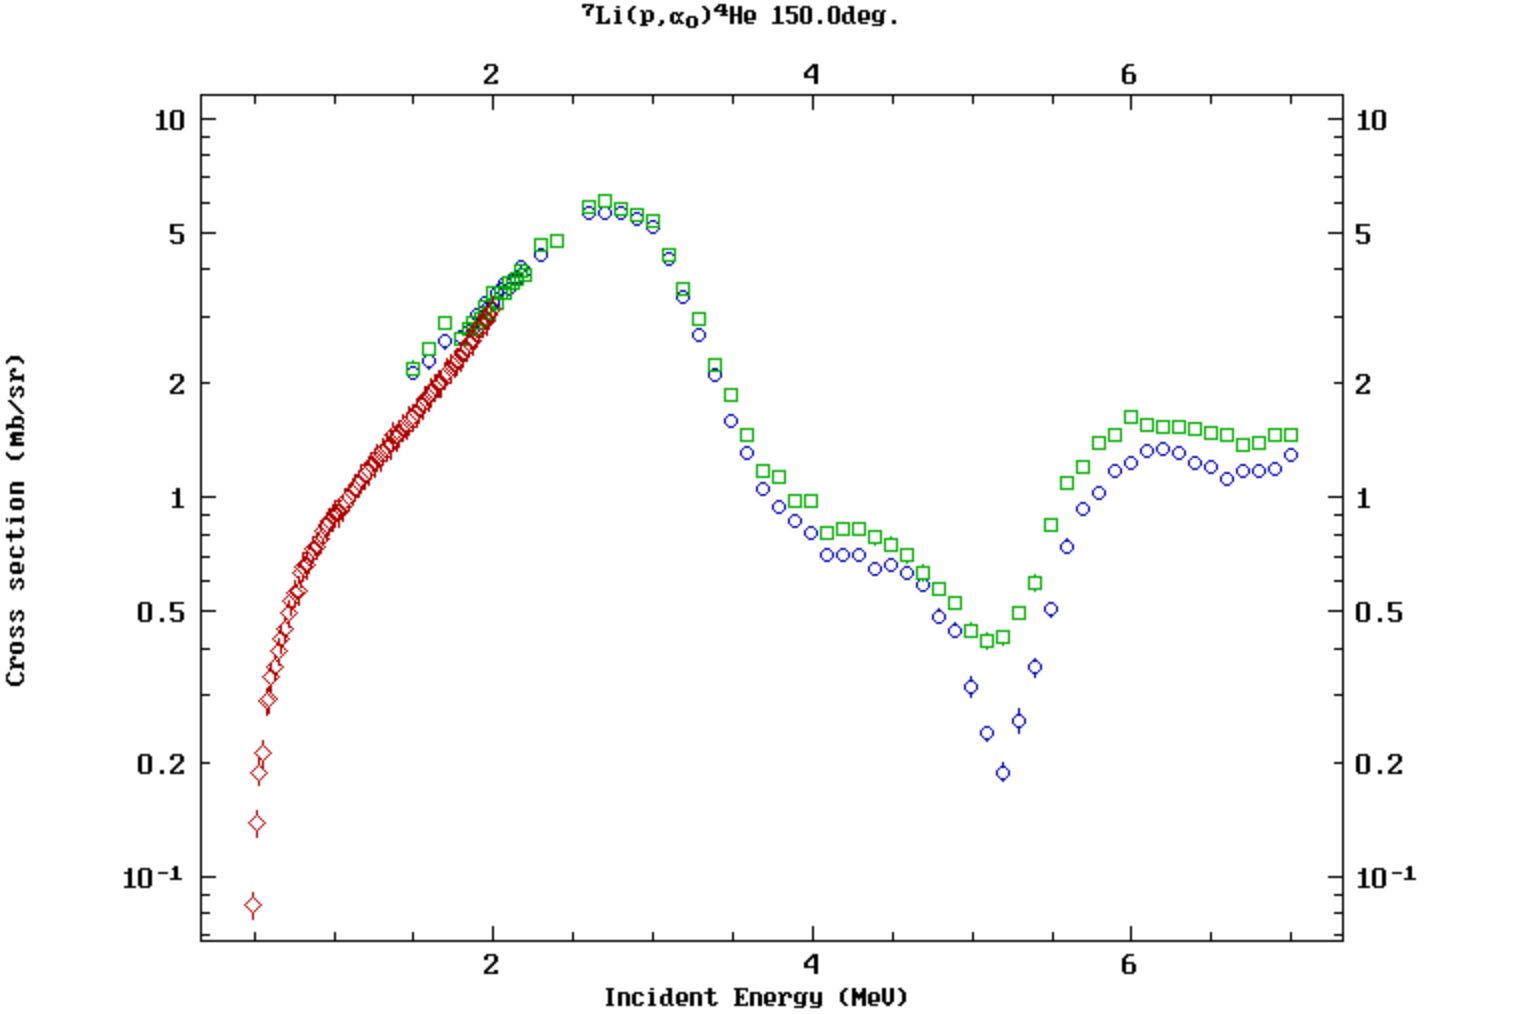
\includegraphics[width=0.95\linewidth]{../images/Li_crosssection_energy.jpeg}
  \captionof{figure}{Cross section of the reaction between protons and Li-7 as a function of the beam energy.}
\end{center}


\section{Safety considerations}

During the experiments, the accelerator will be producing a beam of protons with a kinetic energy of up to 5 MeV. Because of this there will be a high radiation level near the accelerator.
There are radiation maps that show the radiation levels in different areas of the laboratory.

\section{Beamtime requested}

Specify the dates of the beamtime requested and the number of shifts. The beamtime requested should be in accordance with
the estimated duration of the experiment. Specify the place and the investigators who will guide the experiment.

\paragraph*{}

In order to complete our project we will need one full day of beamtime at the CTN laboratory. Alongside this day, we will
also meet with the investigators at CTN for another two mornings to discuss the project, before the experiment and the
results after the experiment:

\begin{table}[H]
\centering
\begin{tabular}{|w{0.4\linewidth}|w{0.3\linewidth}|w{0.15\linewidth}|}
\hline
Phase & Date & Duration \\ \hline
Theoretical Background, Planning and Lab Overview & 30/11/2023 9h30 & 4h \\ \hline
Experiment & 7/12/2023 8h00 & 8h \\ \hline
Results Discussion & ?? 9h30 & 4h \\ \hline
\end{tabular}
\end{table}

\section{Results expected}

Describe the results expected from the measurements, their scientific (or technical) relevance, and how they relate to
existing work on the topic.

\paragraph{}

We expect to obtain the energy spectrum of the alpha particles resulting from the reaction between the protons and the
samples. 
For the glass samples, we expect to see a profile due to the particles that come from different depths of the sample and
therefore have lost different amounts of energy. In the implant samples, we expect to see a peak at the energy corresponding
to the energy of the alpha particles produced by the reaction.
In both cases, the samples is composed by other types of atoms such as silicon and boron, which will also emit charged
particles.

\paragraph{}

Other phenomena such as Rutherford Backscattering and Elastic Scattering are also expected to occur.

\section{Concluding remarks}

Justify the beam time you request and give technical reasons which make the apparatus necessary for your experiment.
Include REFERENCES where these are relevant, but do not assume that they will be systematically consulted for essential
details.

\printbibliography
\nocite{*}

\end{multicols}

\end{document}